\begin{anexosenv}

\partanexos

\chapter{Princípios e Práticas do Lean na Manufatura}

\section[Princípios]{Princípios}

\subsection[Constância de Propósitos]{Constância de Propósitos}

O princípio de Constância de Propósitos diz respeito a manter a clareza dos objetivos importantes de longo prazo e é um dos constituintes da base da pirâmide dos princípios porque prover a persistência necessária para influenciar o comportamento de todos dentro da organização. Quando diariamente o comportamento muda, a cultura da organização também muda. A Constância de Propósitos tem o foco no pensamento e no comportamento, fazendo com que todos caminhem na mesma direção. As pessoas devem ser encorajadas a desafiar o modo como as coisas são feitas e a perceber as dificuldades e oportunidades de melhoria, a partir disso, é possível ter a resolução de problemas de forma colaborativa \cite{bell2011}.

Com isso, líderes executivos têm a responsabilidade de definir objetivos estratégicos e criar constância de propósitos. Os gestores tem como responsabilidade eliminar impedimentos, estabilizar os processos e ajudar os trabalhadores a desenvolver habilidades de resolução de problemas, para que eles possam sentir-se donos do seu trabalho e possam assumir responsabilidade sobre a melhoria contínua  \cite{bell2011}. 


\subsection[Respeito às Pessoas]{Respeito às Pessoas}

O segudo princípio base é o respeito às pessoas. Todos os indivíduos possuem uma única coleção de experiências e fazem distintas contribuições quando participam de um processo de melhoria. A resolução de problemas coletiva só ocorre quando existe respeito pelas pessoas em todos os níveis hierárquicos de uma organização. O respeito direciona o desenvolvimento dos trabalhadores, encoraja participação e melhora a relação entre fornecedor e cliente \cite{bell2011}.

Além disso, respeito às pessoas encoraja alcançar a excelência profissional e o pontêncial criativo. Em um ambiente de aprendizado e desenvolvimento colaborativo as pessoas sabem que suas ideias possuem valor e sentem-se mais estimuladas em melhorar diariamente. Pessoas estimuladas e respeitadas não só geram sucesso individual como também sucesso coletivo e organizacional.


\subsection[Melhoria Contínua e Perfeição]{Melhoria Contínua e Perfeição}

O último princípio da base da pirâmide é a melhoria contínua em busca da perfeição.  As soluções imediadas, emboram possam ser adequadas para hoje, são na melhor das hipóteses temporárias.  A mudança é constante e novas ideias são necessárias  sempre que o padrão de trabalho atual não produz mais os resultados esperados. Em uma cultura Lean, os trabalhadores devem aceitar as mudanças como inevitáveis e de forma proativa enfrentarem os desafios. Cada indivíduo deve ver o seu trabalho como tendo dois componentes inseparáveis: trabalho diário e melhoria diária \cite{bell2011}.

No entanto, as pessoas possuem hábitos diferentes. Muitas pessoas gostam da mudança, mas não gostam de serem mudadas, pois para mudar é preciso sair da zona de conforto.  Com isso, as pessoas costumam resistir a mudanças e impedir que a criatividade e inovação sejam desenvolvidas dentro de si.  Quando Lean é visto como um programa ou projeto, com início e fim, elas costumam aceitar e realizar o que é pedido. Quando o projeto termina, voltam a praticar os mesmo hábitos e comportamentos de antes. Porém, quando coletivamente as pessoas reconhecem que se não estão melhorando, estão ficando para trás, a compreenssão do trabalho diário muda radicalmente. Esta percepção inspira novas ideias e a reinvenção diária, influenciando no sucesso de toda a organização\cite{bell2011}.


\subsection[Comportamento Proativo]{Comportamento Proativo}

O princípio que fica sobre a base da pirâmide é o de comportamento proativo, que significa tomar iniciativa, assumindo pessoal responsabilidade pela qualidade do próprio trabalho e pelo ambiente de trabalho. Ser proativo significa aproveitar a oportunidade para fazer a diferença dia a dia \cite{bell2011}.

Em os 7 Hábitos de Pessoas Altamente Eficazes, o Dr. Stephen Covey introduz um modelo chamado Matriz de Gerenciamento de Tempo, dividindo o trabalho em quatro quadrantes com base na importância e urgência, como ilustrado na Fig. (20).

\begin{figure}[H]
		\centering
		\label{fig03}
			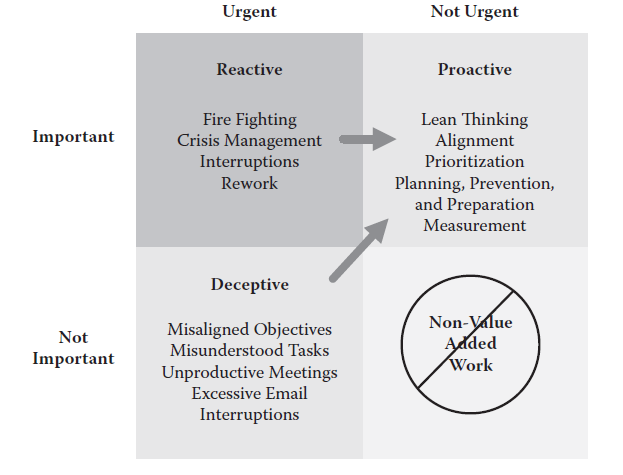
\includegraphics[scale=0.9]{figuras/matrizcomportamento.png}
		\caption{Matriz de Gerenciamento de Tempo \cite{bell2011}}
\end{figure}

Ele ressalta que o trabalho de maior valor encontra-se no quandrante importante e não urgente, onde o planejamento proativo, a prevenção, a preparação e a aprendizagem serão mais fortemente desenvolvidos. Trabalho não planejado concentra-se no quadrante importante e urgente (combate de forma reativa) ou não importante e urgente (atividades que parecem importante devido à sua urgência). Em ambos os casos, eles roubam tempo e recursos que devem ser usados para abordar proativamente o trabalho importante e não urgente. O comportamento reatiavo, geralmente, deixa desperdício e impede o progresso. 

Lean desloca-se da ênfase em sempre realizar trabalho não planejado para o trabalho proativo de melhoria contínua. Esta é uma abordagem eficaz porque quanto mais tempo é gasto na melhoria contínua, menos trabalho não planejado e urgente aparecem e mais tempo é liberado para trabalhar de forma proativa.

O próximo nível da pirâmide está relacionado ao conhecimento em três perspectivas: voz do cliente, qualidade na raíz e pensamento sistêmico.

\subsection[Voz do Cliente]{Voz do Cliente}

A maioria dos processos têm tanto os clientes internos que irão receber os produtos de trabalho e o rendimento deles quanto os clientes externos (parceiros comerciais e usuários finais) que recebem o produto final, serviço ou informação. Para compreender claramente a voz do cliente é preciso estar envolvido com os clientes, seja ele quem for. Ao ouvirmos constantemente a voz do cliente temos a garantia que estamos focados nas questões certas e fazendo melhorias que serão valiosas para os clientes atuais e futuros. Entender as necessidades e os desejos dos clientes mais claramente que o concorrente faz com que a empresa seja mais competitiva e ágil \cite{bell2011}.

\subsection[Qualidade na Raíz]{Qualidade na Raíz}

A qualidade na raíz significa fazer as coisas certas da primeira vez sempre, o trabalho com problemas não é enviado para etapa seguinte ou para o cliente. A abordagem de concertar mais tarde um problema é praticado em muitas organizações devido a pressão do prazo, inadequado treinamento e conhecimento não adequado do processo.  A melhor hora de resolver um problema é no momento que ele acontece, pois a a causa ainda está fresca, os trabalhadores estão atentos e isso previne a adição de defeitos até que a causa do problema seja encontrada.  O foco do trabalho diário deve ser produzir qualidade desde o início \cite{bell2011}.

Em um ambiente Lean existe a obrigação de parar e corrigir problemas e um comprometimento coletivo de não deixar que os defeitos conhecidos cheguem até o cliente. Por meio do trabalho padronizado e do treinamento, todo o esforço é feito para garantir que o problema ou defeito não seja repetido novamente. As pessoas assumem a responsabilidade do trabalho que elas passam adiante, independentemente de onde veio o problema. Essa mudança fundamental na atitude reduz o desperdício e a frustração. Com isso, quando a qualidade na raíz toma conta, mais tempo é disponibilizado para desenvolver o que o cliente está pagando, o que por sua vez melhora a produtividade, custo, qualidade e moral \cite{bell2011}.

\subsection[Pensamento Sistêmico]{Pensamento Sistêmico}

O terceiro elemento do terceiro nível da pirâmide é o pensamento sistêmico: a capacidade de visualizar a interligação entre os processos que compõem a cadeia de valor inteira embora esteja ciente da interdependência de causa e efeito que podem criar valor ou criar desperdícios \cite{bell2011}.

A cadeia de valor é composta de todos os processos, atividades e tarefas usados para gerar um produto ou serviço desde a sua concepção até a sua entrega ao cliente, e inclui todas as informações, procedimentos e materiais. Para evitar soluções que criem otimização localizada, o Pensamento Lean requer conhecimento da natureza de todas as regras de negócio e fluxos de informações.   

Esta não é a forma natural que a mente humana e as organizações trabalham, as pessoas tendem a concentrar-se em partes espcíficas de um quebra-cabeça em vez de concentrar-se em toda a imagem. Medidas inadequadas e os incentivos muitas vezes reforçam essa estreita forma de concentração.

Quando a solução de problemas baseia-se em uma compreensão clara da cadeia de valor global e dos clientes que são atendidos por ela, as empresas evitam o erro comum de realizar melhorias locais, que muitas vezes transferem ineficiências e desperdícios de uma área para a outra. Equipes multifuncionais fornecem a amplitude de entendimento necessário para o pensamento sistêmico, abrangendo o fluxo de valor, ligando o conhecimento e a compreensão de cada membro da equipe.

A perspectiva holística mostrada aqui pode ser desconhecida para muitos profissionais que passaram suas carreiras a aperfeiçoar as habilidades em uma área especializada da empresa. Um pensamento sistêmico estimula o potencial criativo dos trabalhadores, ampliando seus horizontes e desafiando a amplitude de sua percepção. Para fazer melhorias que impactam no que é recebido pelo cliente externo, a cadeia de valor deve ser vista como um sistema. O mapeamento do fluxo de valor e o pensamento sistêmico são complementares, ambos ajudam as pessoas a ver processos de negócios em um novo contexto: fluxo. Assim, o pensamento sistêmico permite ver o todo, criando um fluxo de valor para o cliente \cite{bell2011}.

\subsection[Fluxo Contínuo, Produção Puxada e \textit{Just in Time}]{Fluxo Contínuo, Produção Puxada e \textit{Just in Time}}

O próximo nível da pirâmide concentra-se no fluxo: a progressão ininterrupta de materiais, serviços e informações.  Como Jeffrey Liker enfatiza no “Toyota Way”: "permitir que o trabalho flua sempre que puder, quando o fluxo é interrompido, utilize sinais para puxar o início do trabalho".

O fluxo é conseguido por meio da eliminação de atrasos e interrupções durante toda a cadeia de valor. O mapeamento do fluxo de valor é uma ferramenta eficaz para identificar, quantificar e eliminar o desperdício. O fluxo de informações produz a transparência e visibilidade necessária para coordenar de forma eficiente o fluxo de trabalho. Quando a informação é usada para nivelar a demanda, equilibrar a capacidade e melhorar a qualidade, o fluxo é melhorado e valor é entregue ao cliente de forma rápida. Quando não há interrupções em uma série de tarefas, o trabalho flui sem problemas. Tipicamente, o trabalho irá fluir até encontrar uma barreira que impeça sua continuidade, por exemplo, o transporte para o outro local \cite{bell2011}. 

A produção puxada diz respeito ao cliente puxar a cadeia de valor. Ou seja, o cliente determina qual é o produto que ele deseja. Com isso, a produção é feita sobre demanda. A produção em massa deveria ser eliminada, pois ela empurra o produto para o cliente sem que ele tenha oportunidade de decidir o que realmente deseja. Assim, a produção puxada inverte o valor produtivo: as empresas não mais empurram os produtos para o consumidor por meio de descontos e promoções. O consumidor é que passa a “puxar o fluxo do valor”, reduzindo estoques e valorizando o produto \cite{bell2011}.

O \textit{Just in Time} como dito na seção anterior é um dos pilares do Pensamento Lean e estar relacionado aos dois conceitos anteriores. Ele tem como objetivo eliminar todas as fontes de desperdício e tudo o que não acrescenta valor à organização. O princípio para atingir este fim é simples: só produzir o que é pedido pelo cliente e só quando ele o pretende, ou seja, não manter estoques, seja de produtos acabados ou intermediários. 

\subsection[Cultura]{Cultura}

O princípio localizado no topo da pirâmide é a cultura: ela representa crenças compartilhadas de uma organização e o valor,  os quais manifestam-se na atitude e no comportamento dos membros da organização. Cultura é o resultado da mudança de comportamento, em Lean ela está relacionada a melhoria contínua e a proatividade das pessoas na resolução de problemas. A mudança cultural pode resultar em um desempenho superior, na vantagem competitiva e em bons resultados financeiros \cite{bell2011}.

A evolução de uma cultura Lean geralmente começa com adoção de práticas de melhoria contínua, seguida pela formação de um comportamento orientado a sistemas e orientado por valores e princípios comuns. As práticas do Lean fornecem estrutura e capacitação. Os sistemas desenvolvem práticas em comum. E os princípios fornecem a base que reforça os padrões culturais e o comportamento diário.

\section[Conceitos de Valor e Desperdício]{Conceitos de Valor e Desperdício}

O principal foco do Lean é a resolução de problemas com o propósito de entregar valor ao cliente, com base na sistemática eliminação de desperdícios ao longo do fluxo ou da cadeia de valor. Portanto, esses três conceitos: valor, fluxo de valor e desperdícios precisam estar claros.

Para um entendimento mais conciso do Pensamento Lean é importante ainda ter em mente que o termo desperdício recebe uma conotação específica e uma autêntica subordinação à ideia de valor. Ou mais especificamente, ao valor percebido pelos clientes, considerando suas expectativas, necessidades e desejos. A melhor maneira para se identificar os desperdícios, segundo o pensamento Lean, é colocar-se na posição do cliente e refletir criticamente sobre os processos de produção na forma como são realmente feitos \cite{costa2010}.

\subsection[Valor]{Valor}

O ponto de partida para o Pensamento Lean consiste em definir o que é valor e o fluxo do valor. Diferente do que muitos pensam, não é a empresa, e sim o cliente quem define o que é valor. Para ele, a necessidade gera o valor e cabe às empresas determinarem qual é essa necessidade. A partir disso, pode-se procurar satisfazer esssa necessidade e cobrar um preço específico sobre ela \cite{leaninstitute}. Assim, valor é aquilo que o cliente deseja e pelo que ele paga. 

\subsection[Cadeia de Valor]{Cadeia de Valor}

O fluxo de valor é composto por todo o ciclo de vida dos processos requeridos para gerar serviços, produtos e informação do conceito ao cliente.  Isto incluí todas as atividades, que criam ou não valor. O pensamento sistêmico ajuda as pessoas a perceberem o processo e entender o valor da perspectiva do cliente. 

Para isso, é preciso dissecar a cadeia produtiva e separar os processos em três tipos: os que efetivamente geram valor, aqueles que não geram valor, mas são importantes para a manutenção do processo e para a qualidade do processo e do produto, e aqueles que não agregam valor e que devem ser eliminados (os desperdícios) \cite{leaninstitute}.

\subsection[Os Três Ms]{Os Três Ms}

De acordo com o Lean, os desperdícios podem ser divididos em três categorias, conhecidas como os três Ms: mura, muri e muda. O Mura significa irregularidade e variação, ele representa a inconsistência no fluxo de trabalho causada pelas mudanças, variedade e qualidade desejadas pelo cliente. É preciso saber minimizar os impactos causados pelo mura por meio da padronização do processo. O Muri significa sobrecarga, que representa a carga excessiva sobre as pessoas ou sobre os equipamentos, o que pode causar stress, erros e retrabalho. É preciso saber remover sobrecargas por meio da padronização do processo e gerenciamento adequado da demanda. E o Muda, que diz respeito ao desperdício em si, o qual na produção da Toyota foram categorizados em sete tipos: superprodução, estoque, tempo de espera, transporte, processos inadequados, movimentação de pessoas e correção devido à defeitos  \cite{bell2011}.

\section[Práticas e Ferramentas]{Práticas e Ferramentas}

O Pensamento Lean sugere um conjunto de práticas e ferramentas que podem ser aplicadas na organização a fim de atingir os objetivos defendidos por ele. Vale ressaltar que as práticas aqui apresentadas são aquelas consideradas principais para este trabalho, a organização deve buscar aquelas que melhor se adeque ao seu contexto. Como dito anteriormente, as ferramentas servem de estrutura e meio de capacitação, é importante que os trabalhadores, sobretudo, vivam diariamente os princípios da cultura Lean.

\subsection[A3 Thinking]{A3 Thinking}

O pensamento A3 é a aplicação consistente do PDCA(\textit{Plan, Do, Check and Act}) na resolução de problemas para identificar o melhor caminho para enfrentar desafios e oportunidades. O pensamento A3 guia as atividades da equipe em direção a uma correta definição dos problemas ou oportunidades. A ferramenta usada no pensamento A3 é o relatório A3, que se refere a um formato padronizado de comunicação que expressa o processo de resolução de problema em uma folha de papel em tamanho A3.

O uso de apenas uma folha para expressar todo o conhecimento faz com que as pessoas refinem seus pensamentos de modo que todas as questões e soluções sejam expostas de forma simples \cite{liker}. 

\subsection[Mapeamento da Cadeia de Valor]{Mapeamento da Cadeia de Valor}

O mapeamento da cadeia de valor é uma das ferramentas mais utilizados no Lean, ele permite identificar todas as atividades de um processo da organização que criam ou não criam valor do ponto de vista do cliente, ou seja, permite visualizar todo o fluxo, ao longo da cadeia de valor, desde a concepção até à entrega ao cliente \cite{bell2011}.

O mapeamento do fluxo de valor representa visualmente o fluxo de informações e materiais com ênfase na quantificação de desperdícios e na quantificação de tempo e qualidade. Ele pode ser feito com grande nível de detalhe, porém, tipicamente, o foco está em um nível mais macro do que no mapeamento de processos  e não inclui tarefas e decisões individuais.

\subsection[Kaizen]{Kaizen}

O Kaizen é uma das práticas sugeridas pelo Lean. A palavra Kaizen é a junção de duas palavras japonesas: Kai que significa mudança e Zen que significa bom, porém é comum traduzi-la para melhoria contínua. O Kaizen  pode ser considerado uma forma de atingir os objetivos do Lean \cite{bell2011}.

Esta melhoria é obtida por todos os trabalhadores e tem foco na eliminação de todo tipo de desperdício. Apesar de este ser um processo lento e incremental, os ganhos em longo prazo são grandes.

Um dos conceitos utilizados pelo Kaizen é a metodologia PDCA, desenvolvido por William Edwards Deming. Esta metodologia é composta por quatro etapas:
\begin{itemize}
\item Planejar: refere-se à definição do problema, bem como suas possíveis causas e soluções, o estabelecimento de um plano corretivo e os objetivos de forma clara;
\item Fazer: refere-se à implementação do plano e à recolha dos dados para análise;
\item Verificar: refere-se a verificar se os dados recolhidos vão de encontro aos objetivos definidos e é feito o registro dos resultados;
\item Agir:  é onde são padronizados os resultados que foram eficazes e, se houver medidas não eficazes, o ciclo é refeito.
\end{itemize}

Assim, o Kaizen é um processo incremental e contínuo que abrange toda a organização e o envolvimento de todos os trabalhadores. Todos devem trabalhar de forma proativa em busca da melhoria diária e acreditar que bons resultados virão em longo prazo.

\subsection[Metodologia 5S]{Metodologia 5S}

Os 5S pode ser considerada a ferramenta mais básica que o Lean sugere, é considerado um passo a mais em direção à melhoria da qualidade e da produtividade. O objetivo desta prática é organizar o ambiente de trabalho de forma adequada para que o trabalhador tenha, apenas, os materiais e ferramentas necessários para executar seu trabalho \cite{bell2011}. 

O nome desta metodologia é originado de cinco palavras japonesas: Seiri, Seiton, Seiso, Seiketsu e Shitsuke. Para que o método funcione é preciso que as pessoas realmente entendam a importância dele e que ele seja um processo rotineiro e não apenas aplicado de forma isolada.

O primeiro conceito, Seiri, consiste na  remoção de todos os materiais e ferramentas não necessários para a executação das tarefas diárias, é importante que os itens sejam identificados por frequência de utilização para que sua prioridade seja percebida.  O segundo conceito, Seiton, consiste na organização dos itens de trabalho, de forma que eles estejam acessíveis ao trabalhador de forma rápida, aumentando a eficácia e  a eficiência das atividades, os itens devem estar alocados em lugares próximos e instalados e configurados no ambiente de trabalho de forma correta, no caso de \textit{softwares}. O terceiro conceito, Seiso, consiste na limpeza do local de trabalho diariamente, proporcionando um ambiente confortável, limpo e ergonômico. O quarto conceito, Seiketsu, consiste na padronização e sistematização de todas as atividades ditas anteriormente, de forma que esteja disponível para todos os trabalhadores. E o quinto conceito, Shitsuke, diz respeito à sustentabilidade e à disciplina. Para que os resultados sejam visíveis em longo prazo existe a necessidade de acompanhamento e disciplina. Quando um problema é identificado não se deve julgar ou culpar os trabalhadores, mais sim realizar reuniões para que o problema seja resolvido de forma colaborativa e harmoniosa  \cite{bell2011}. 

\subsection[Kanban]{Kanban}

Uma das ferramentas de grande importância associado ao Pensamento Lean é o sistema Kanban (Fig. 21) , palavra japonesa que significa cartão ou registro visível. Sendo mais um dos conceitos desenvolvidos pela Toyota, este sistema tem como objetivo o balanceamento da produção e a minimização de estoque. Por meio da gestão visual, os Kanbans fornecem de forma simples e intuitiva indicações aos trabalhadores relativas a fluxos de materiais, recursos e informação. 

Este sistema é implementado com o objetivo de atingir a produção \textit{Just-in-Time}, ou seja, produzir na quantidade certa, na altura devida e o produto correto. O Kanban limita o trabalho em progress, o que fornece previsibilidade de tempo em ciclos e faz com que as entregas sejam mais confiáveis. A abordagem de "parar a linha de produção", para superar os obstáculos e os erros encontrados, também resulta em níveis mais elevados de qualidade e uma queda rápida de retrabalho. Além disso, o Kanban implica um modelo de produção do tipo \textit{pull}, ou seja, este sistema desencadeia ordens de produção vindas do cliente\cite{rodrigues2012}.  

\begin{figure}[H]
		\centering
		\label{fig04}
			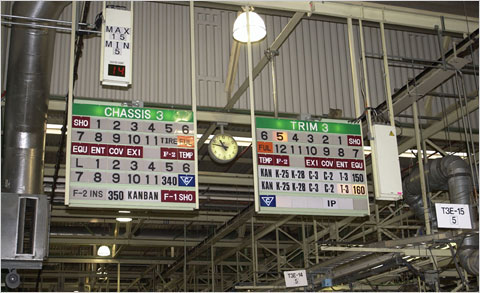
\includegraphics[scale=1.0]{figuras/kanbanindustria.png}
		\caption{Quadro Andon, com o mesmo objetivo do Kanban, na fábrica da Toyota \cite{kanbanindustria}}
\end{figure}

\chapter{Metodologia IPHAN de Gestão de Demandas de Desenvolvimento Ágil de \textit{Software}}

O MIDAS foi baseado nos príncipios ágeis advindos do Manifesto Ágil, tais princípios foram adaptados ao contexto do órgão. Os princípios norteadores deste modelo foram:
\begin{itemize}
\item Envolvimento do requisitante (cliente): as áreas requisitantes devem estar profundamente envolvidas no processo de desenvolvimento. Seu papel será fornecer e priorizar novos requisitos dos sistemas e avaliar as iterações;
\item Entrega incremental: o \textit{software} é desenvolvido em incrementos e o cliente especifica os requisitos a serem incluídos em cada incremento;
\item Foco nos resultados e não no processo: a equipe de desenvolvimento deve desenvolver suas próprias maneiras de trabalhar, sem processos prescritivos;
\item Aceitação de mudanças: ter em mente que os requisitos de um sistema podem mudar fará com este seja projetado para acomodar as mudanças;
\item Manter a simplicidade: sempre que possível, a complexidade de um sistema deve ser eliminada concentrando-se na simplicidade tanto do sistema quanto do processo de desenvolvimento.
\end{itemize}

Os papéis definidos no MIDAS são: área de TI, área de negócio (requisitante) e o fornecedor contratado. Ao relacionamos estes papéis com os papéis do Scrum temos de forma geral que os representantes da área requisitante serão o \textit{Product Owner}, um representante da área de TI do órgão e um representante do fornecedor representarão o papel de Scrum \textit{Master} e a equipe do fornecedor contratado representa a Equipe de Desenvolvimento do Scrum. Se mapearmos ainda os papéis do Scrum com os papéis específicos definidos pela IN 04, temos como resultado a Tab. (4). 

\begin{table}[H]
\center
\footnotesize
\begin{tabular}{|p{6cm}|p{6cm}|}
  \hline
   \textbf{Papéis MIDAS/SCRUM} & \textbf{Papéis IN 04/2010}\\
    \hline
   Product Owner & Área Requisitante da Solução, Integrante Requisitante, Fiscal Requisitante, Gestor do Contrato\\
   \hline    
    Scrum Master IPHAN & Área de TI, Integrante Técnico, Fiscal Técnico, Gestor do Contrato\\
    \hline
   Scrum Master Contratada & Preposto\\
   \hline
    Equipe de Desenvolvimento & Equipe do fornecedor contratado\\
   \hline
\end{tabular}
\caption{Papéis MIDAS x Papéis IN 04}
\end{table}

As demandas para desenvolvimento de sistemas são divididas em cinco tipos dentro do MIDAS: sistema novo, manutenção evolutiva, manutenção corretiva, documentação de sistemas legados e refatoração.  O sistema novo e a manutenção evolutiva devem seguir todo o processo do MIDAS. A refatoração e a documentação de sistemas legados podem seguir todo o processo do MIDAS ou apenas o subprocesso Sprint. Já a manutenção corretiva não segue nenhum dos processos, ela seguirá uma ordem de serviço específica de acordo com sua urgência.

O processo MIDAS é dividido em três fases: planejamento, desenvolvimento e encerramento, e deve ser executado de forma incremental, com entregas frequentes e progresso medido continuamente. O macro fluxo do processo MIDAS é representado pela Fig. (22).

\begin{figure}[H]
		\centering
		\label{fig01}
			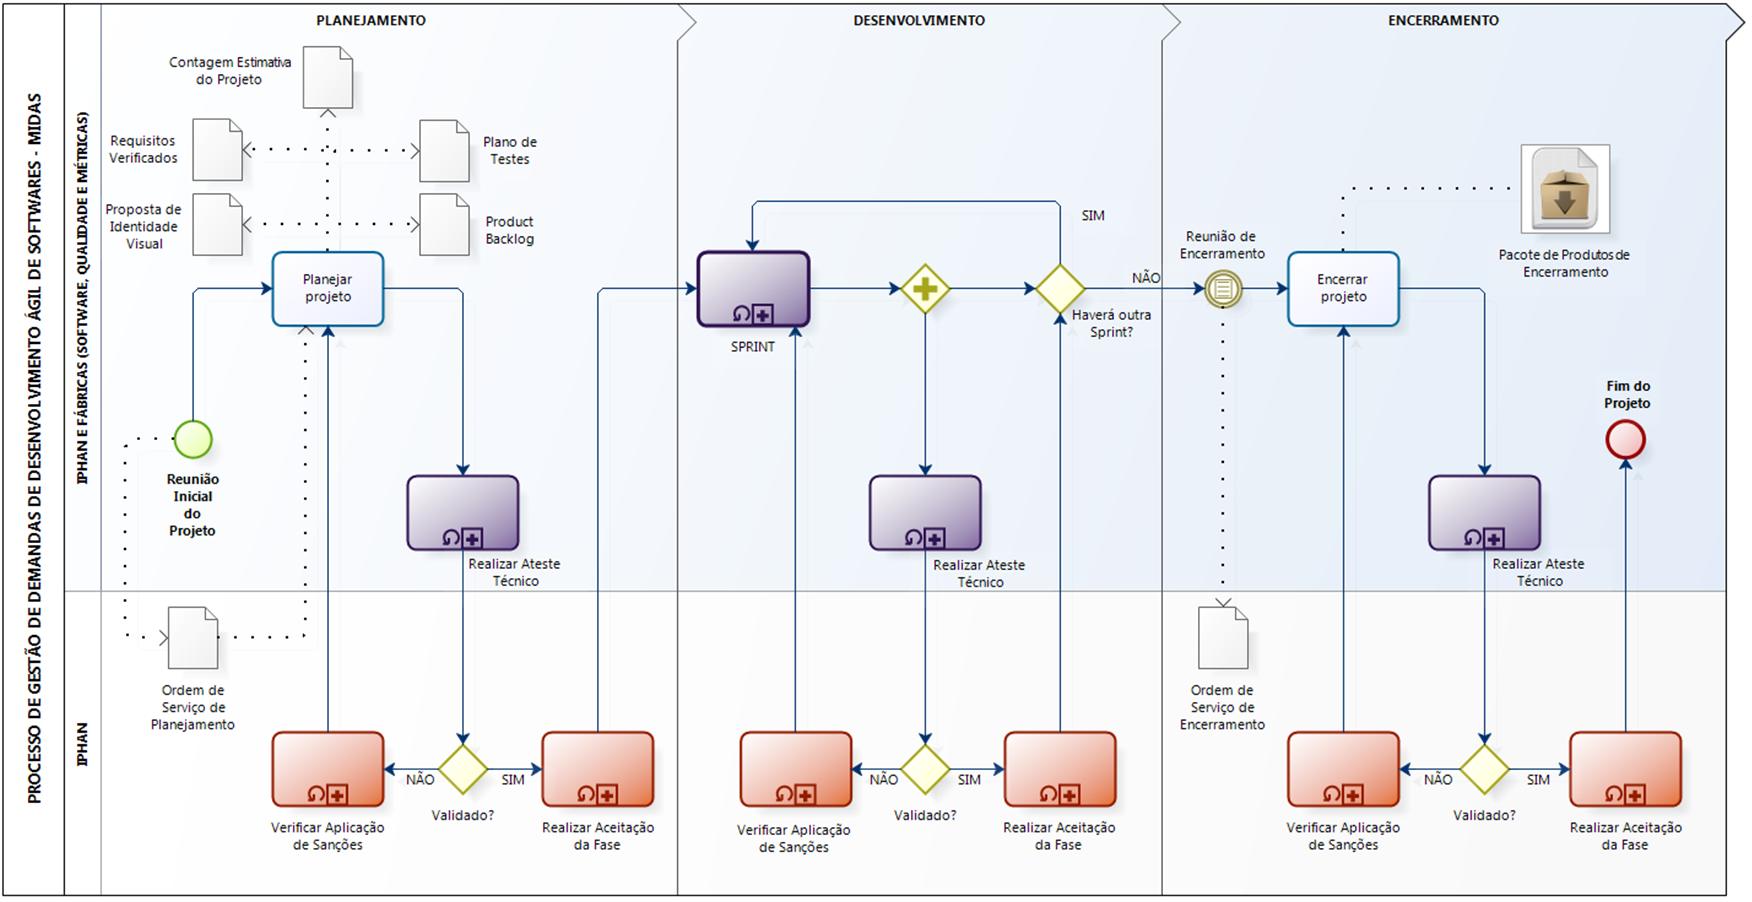
\includegraphics[scale=0.3]{figuras/processoMIDAS.png}
		\caption{Processo MIDAS \cite{IPHAN:2013}}
\end{figure}

O primeiro subprocesso advindo do planejamento é o subprocesso Realizar Ateste Técnico, trata-se de um subprocesso padrão que será executado em todas as fases do processo MIDAS. Nele estão contidos outros dois processos: Medição de Sistemas e Controle de Qualidade, cujo detalhamento não cabe no escopo deste trabalho. O subprocesso de Realizar Ateste Técnico tem o objetivo de verificar se os requisitos de cada fase foram satisfeitos e se os produtos de trabalho atendem às especificações de entrada e aos planos e regras estabelecidos. O fluxo deste subprocesso está representado na Fig. (23) com suas atividades, entradas e saídas.

\begin{figure}[H]
		\centering
		\label{fig01}
			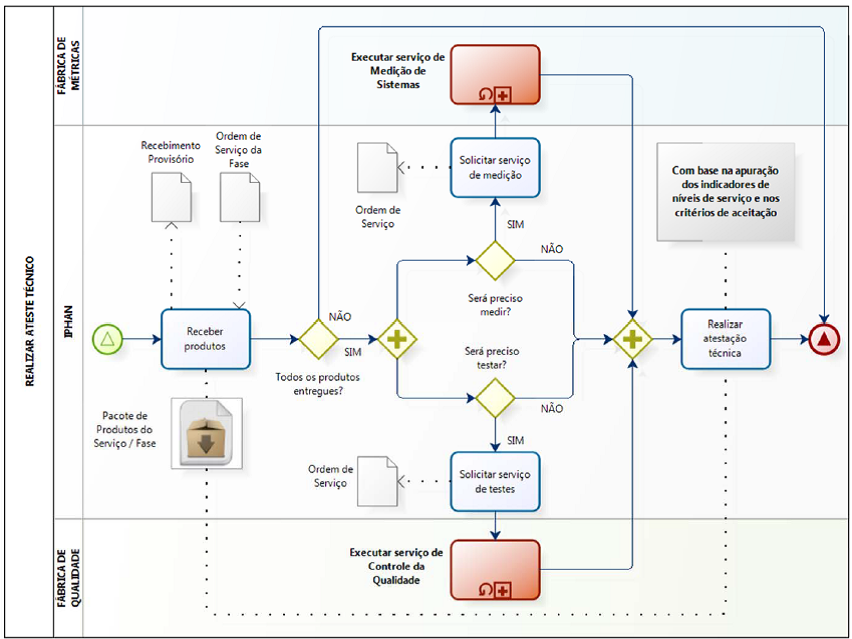
\includegraphics[scale=0.7]{figuras/subprocessoAteste.png}
		\caption{Subprocesso Realizar Ateste Técnico \cite{IPHAN:2013}}
\end{figure}

O subprocesso Sprint é o principal processo da fase de desenvolvimento e tem o objetivo de realizar o ciclo de trabalho de desenvolvimento. Sprint é um ciclo de desenvolvimento onde requisitos são implementados tendo como resultado um incremento do produto que está sendo desenvolvido. A quantidade de ciclos totais do projeto é definida na atividade de “Planejar Projeto”, a qual é realizada na fase de planejamento. O fluxo deste subprocesso está ilustrado na figura 24.


\begin{figure}[H]
		\centering
		\label{fig01}
			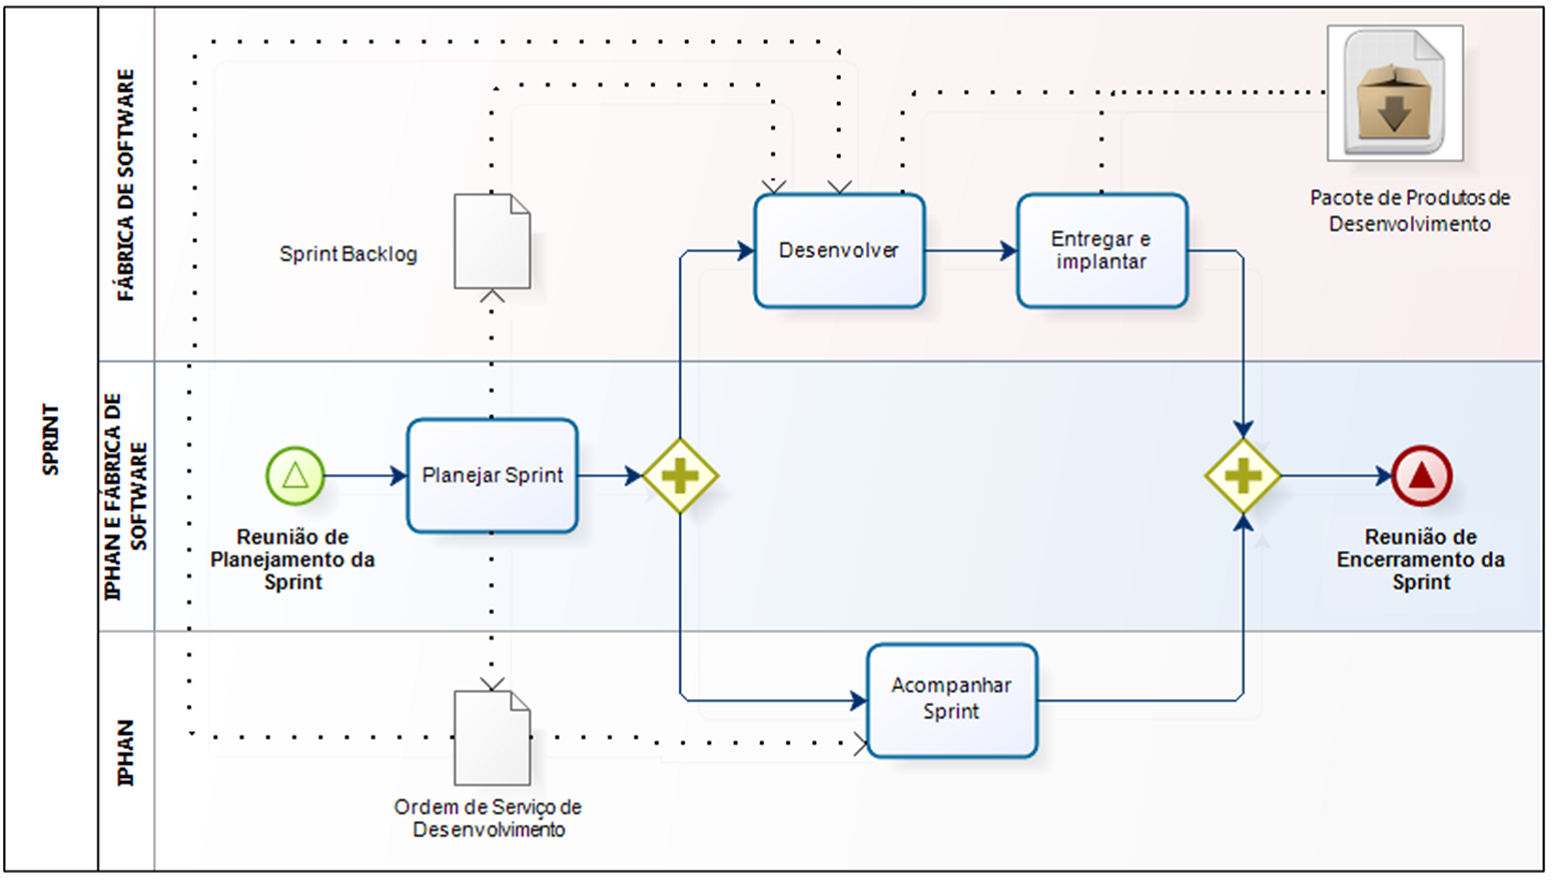
\includegraphics[scale=0.4]{figuras/subprocessoSprint.png}
		\caption{Subprocesso Sprint \cite{IPHAN:2013}}
\end{figure}

\end{anexosenv}

